\documentclass{latex/CUP-JNL-DAP}%


%%%% Packages
\usepackage{graphicx}
\usepackage{multicol,multirow}
\usepackage{amsmath,amssymb,amsfonts}
\usepackage{mathrsfs}
\usepackage{amsthm}
\usepackage{apacite}
\usepackage{rotating}
\usepackage{appendix}
\usepackage[numbers]{natbib}
\usepackage{ifpdf}
\usepackage[T1]{fontenc}%
\usepackage{times}%
\usepackage{sourcesanspro}%
\usepackage{newtxmath}%
\usepackage{textcomp}%
\usepackage{xcolor}
\usepackage{hyperref}
%%%%


% for quarto

\usepackage{fancyvrb}
\usepackage{framed}
\usepackage{calc}
\usepackage{tabularx}
\usepackage{booktabs}
\usepackage{longtable}
\usepackage{float}

\providecommand{\tightlist}{%
  \setlength{\itemsep}{0pt}\setlength{\parskip}{0pt}}
  
\NewDocumentCommand\citeproctext{}{}
\NewDocumentCommand\citeproc{mm}{%
  \begingroup\def\citeproctext{#2}\cite{#1}\endgroup}
\makeatletter
 % allow citations to break across lines
 \let\@cite@ofmt\@firstofone
 % avoid brackets around text for \cite:
 \def\@biblabel#1{}
 \def\@cite#1#2{{#1\if@tempswa , #2\fi}}
\makeatother

\newlength{\cslhangindent}
\setlength{\cslhangindent}{1.5em}
\newlength{\csllabelwidth}
\setlength{\csllabelwidth}{3em}
\newenvironment{CSLReferences}[2] % #1 hanging-indent, #2 entry-spacing
 {\begin{list}{}{%
  \setlength{\itemindent}{0pt}
  \setlength{\leftmargin}{0pt}
  \setlength{\parsep}{0pt}
  % turn on hanging indent if param 1 is 1
  \ifodd #1
   \setlength{\leftmargin}{\cslhangindent}
   \setlength{\itemindent}{-1\cslhangindent}
  \fi
  % set entry spacing
  \setlength{\itemsep}{#2\baselineskip}}}
 {\end{list}}
\newcommand{\CSLBlock}[1]{\hfill\break#1\hfill\break}
\newcommand{\CSLLeftMargin}[1]{\parbox[t]{\csllabelwidth}{\strut#1\strut}}
\newcommand{\CSLRightInline}[1]{\parbox[t]{\linewidth - \csllabelwidth}{\strut#1\strut}}
\newcommand{\CSLIndent}[1]{\hspace{\cslhangindent}#1}

\newcommand{\VerbBar}{|}
\newcommand{\VERB}{\Verb[commandchars=\\\{\}]}
\DefineVerbatimEnvironment{Highlighting}{Verbatim}{commandchars=\\\{\}}
\definecolor{shadecolor}{RGB}{248,248,248}
\newenvironment{Shaded}{\begin{snugshade}}{\end{snugshade}}
\newcommand{\AlertTok}[1]{\textcolor[rgb]{0.94,0.16,0.16}{#1}}
\newcommand{\AnnotationTok}[1]{\textcolor[rgb]{0.56,0.35,0.01}{\textbf{\textit{#1}}}}
\newcommand{\AttributeTok}[1]{\textcolor[rgb]{0.77,0.63,0.00}{#1}}
\newcommand{\BaseNTok}[1]{\textcolor[rgb]{0.00,0.00,0.81}{#1}}
\newcommand{\BuiltInTok}[1]{#1}
\newcommand{\CharTok}[1]{\textcolor[rgb]{0.31,0.60,0.02}{#1}}
\newcommand{\CommentTok}[1]{\textcolor[rgb]{0.56,0.35,0.01}{\textit{#1}}}
\newcommand{\CommentVarTok}[1]{\textcolor[rgb]{0.56,0.35,0.01}{\textbf{\textit{#1}}}}
\newcommand{\ConstantTok}[1]{\textcolor[rgb]{0.00,0.00,0.00}{#1}}
\newcommand{\ControlFlowTok}[1]{\textcolor[rgb]{0.13,0.29,0.53}{\textbf{#1}}}
\newcommand{\DataTypeTok}[1]{\textcolor[rgb]{0.13,0.29,0.53}{#1}}
\newcommand{\DecValTok}[1]{\textcolor[rgb]{0.00,0.00,0.81}{#1}}
\newcommand{\DocumentationTok}[1]{\textcolor[rgb]{0.56,0.35,0.01}{\textbf{\textit{#1}}}}
\newcommand{\ErrorTok}[1]{\textcolor[rgb]{0.64,0.00,0.00}{\textbf{#1}}}
\newcommand{\ExtensionTok}[1]{#1}
\newcommand{\FloatTok}[1]{\textcolor[rgb]{0.00,0.00,0.81}{#1}}
\newcommand{\FunctionTok}[1]{\textcolor[rgb]{0.00,0.00,0.00}{#1}}
\newcommand{\ImportTok}[1]{#1}
\newcommand{\InformationTok}[1]{\textcolor[rgb]{0.56,0.35,0.01}{\textbf{\textit{#1}}}}
\newcommand{\KeywordTok}[1]{\textcolor[rgb]{0.13,0.29,0.53}{\textbf{#1}}}
\newcommand{\NormalTok}[1]{#1}
\newcommand{\OperatorTok}[1]{\textcolor[rgb]{0.81,0.36,0.00}{\textbf{#1}}}
\newcommand{\OtherTok}[1]{\textcolor[rgb]{0.56,0.35,0.01}{#1}}
\newcommand{\PreprocessorTok}[1]{\textcolor[rgb]{0.56,0.35,0.01}{\textit{#1}}}
\newcommand{\RegionMarkerTok}[1]{#1}
\newcommand{\SpecialCharTok}[1]{\textcolor[rgb]{0.00,0.00,0.00}{#1}}
\newcommand{\SpecialStringTok}[1]{\textcolor[rgb]{0.31,0.60,0.02}{#1}}
\newcommand{\StringTok}[1]{\textcolor[rgb]{0.31,0.60,0.02}{#1}}
\newcommand{\VariableTok}[1]{\textcolor[rgb]{0.00,0.00,0.00}{#1}}
\newcommand{\VerbatimStringTok}[1]{\textcolor[rgb]{0.31,0.60,0.02}{#1}}
\newcommand{\WarningTok}[1]{\textcolor[rgb]{0.56,0.35,0.01}{\textbf{\textit{#1}}}}

\usepackage{graphicx}
\makeatletter
\newsavebox\pandoc@box
\newcommand*\pandocbounded[1]{% scales image to fit in text height/width
  \sbox\pandoc@box{#1}%
  \Gscale@div\@tempa{\textheight}{\dimexpr\ht\pandoc@box+\dp\pandoc@box\relax}%
  \Gscale@div\@tempb{\linewidth}{\wd\pandoc@box}%
  \ifdim\@tempb\p@<\@tempa\p@\let\@tempa\@tempb\fi% select the smaller of both
  \ifdim\@tempa\p@<\p@\scalebox{\@tempa}{\usebox\pandoc@box}%
  \else\usebox{\pandoc@box}%
  \fi%
}
% Set default figure placement to htbp
\def\fps@figure{htbp}
\makeatother
%

\articletype{RESEARCH ARTICLE}
\jname{Data \& Policy}
\artid{Pending}
\jyear{2025}
\jmonth{1}
\jvol{Pending}
\jissue{Pending}
\jdoi{10.1017/dap.2025.Pending}
\raggedbottom

\begin{document}

\begin{Frontmatter}

\title[Quarto Template]{Quarto Template}

\author*[1]{Mauricio Vargas
Sepúlveda}\email{m.sepulveda@mail.utoronto.ca}\orcid{0000-0003-1017-7574}
% \author[2]{ }

\authormark{Mauricio Vargas Sepúlveda \etal}

\address*[1]{\orgdiv{Department of Political Science and Munk School of
Global Affairs and Public Policy}, \orgname{University of
Toronto}, \orgaddress{\street{1 Devonshire Place}, \postcode{M5S
3K7}, \state{Toronto, Ontario}, \country{Canada}}}
\address[2]{\orgdiv{}}

\received{Pending}
\revised{Pending}
\accepted{Pending}

\keywords{Template; Quarto; LaTeX; R}

\abstract{This is a template for users that create their plots/tables
with R and would like to avoid copying and pasting results into LaTeX.}

\begin{policy}
To be determined. Write policy relevant articles using R and Quarto.
\end{policy}

\end{Frontmatter}

\section{Introduction}\label{introduction}

Write your introduction here. This template uses Posit PBC (2025).

Consider the following table:

\begin{longtable}[]{@{}rrr@{}}
\caption{Average miles per gallon and horse power for the mtcars
dataset.}\tabularnewline
\toprule\noalign{}
Cylinders & Mean MPG & Mean HP \\
\midrule\noalign{}
\endfirsthead
\toprule\noalign{}
Cylinders & Mean MPG & Mean HP \\
\midrule\noalign{}
\endhead
\bottomrule\noalign{}
\endlastfoot
4 & 26.66364 & 82.63636 \\
6 & 19.74286 & 122.28571 \\
8 & 15.10000 & 209.21429 \\
\end{longtable}

Also consider this image

\begin{figure}[H]

{\centering 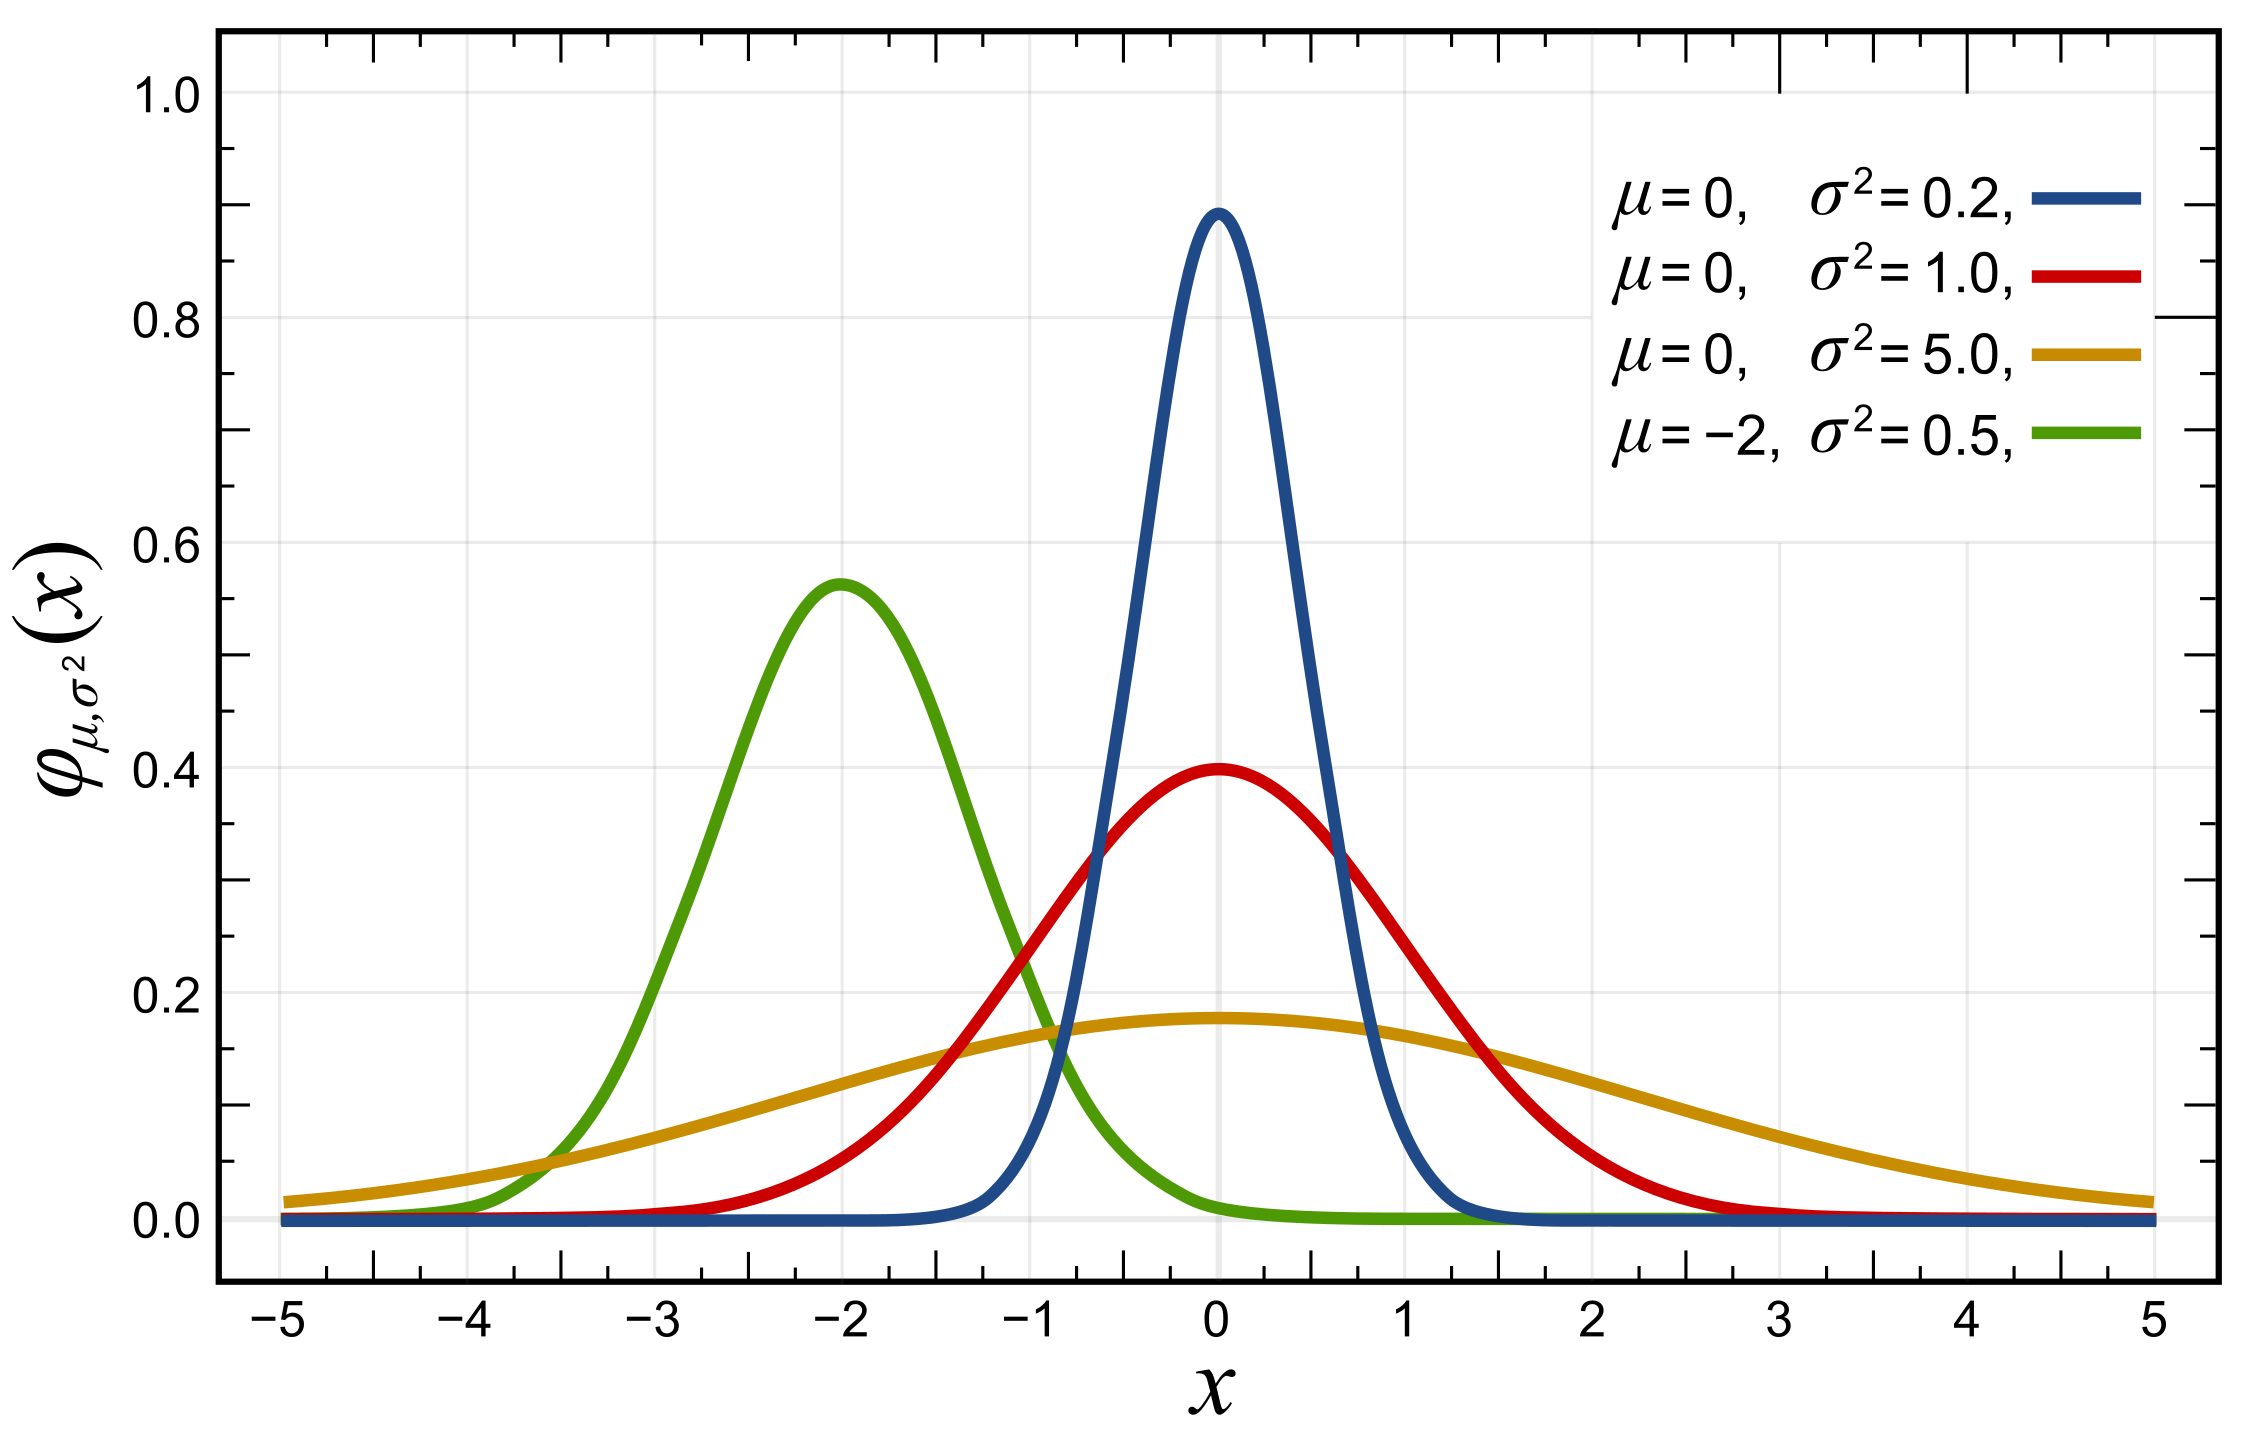
\includegraphics[width=0.5\linewidth,height=\textheight,keepaspectratio]{images/Normal_Distribution_PDF.png}

}

\caption{Normal distribution from Wikipedia}

\end{figure}%

And this R plot

\begin{figure}[H]

{\centering 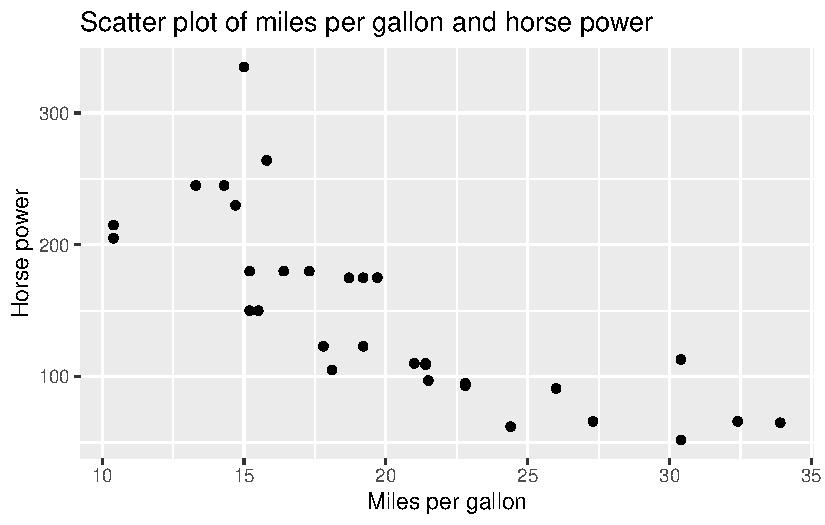
\includegraphics[width=0.5\linewidth,height=\textheight,keepaspectratio]{paper_files/figure-pdf/intro3-1.pdf}

}

\caption{Using ggplot}

\end{figure}%

\section{Content}\label{content}

Write it here.

\section{Access to source code and
data}\label{access-to-source-code-and-data}

Any interested user can explore the source code on
\href{https://github.com/pachadotdev/data-and-policy-quarto-template}{GitHub}
and propose improvements to the template.

\section{Conclusion}\label{conclusion}

I hope it's useful.

\section*{References}\label{references}
\addcontentsline{toc}{section}{References}

\phantomsection\label{refs}
\begin{CSLReferences}{1}{0}
\bibitem[\citeproctext]{ref-posit_pbc_quarto_2025}
Posit PBC. 2025. {``Quarto.''} \emph{Quarto}. \url{https://quarto.org/}.

\end{CSLReferences}

\begin{Backmatter}

\paragraph{Acknowledgments}
Quarto is very convenient to write scientific documents.

\paragraph{Funding Statement}


\paragraph{Competing Interests}
The author declares no competing interests.

\paragraph{Data Availability Statement}
Template fully available here:
https://github.com/pachadotdev/data-and-policy-quarto-template

\paragraph{Ethical Standards}
This template did not involve undue access to data or any other ethical
concerns.

\paragraph{Author Contributions}
Mauricio Vargas Sepúlveda downloaded the official CUP template and
adapted it for Data \& Policy.

% \paragraph{Supplementary Material}
% State whether any supplementary material intended for publication has been provided with the submission.

\bibliographystyle{apalike}
% \bibliographystyle{plainnat}
\bibliography{Sample-refs}

\end{Backmatter}

\end{document}
